\section{ATLAS}

, \cite{collaboration_2020}, \cite{Owen:2302730} 






\subsection*{Data collection}
The ATLAS detector three selection stages before the data is stored. In order to reach the highest intensity of collisions, the LHC accellerates
packets of around $10^{11}$ protons, and collides them at a rate of 25 nanoseconds, yeilding a collision rate of 40 MHz\cite{Wang:2707056}. \cite{Bernius:2707054}

\subsubsection*{Triggers}


\subsubsection*{Data preparation}

\begin{figure}
    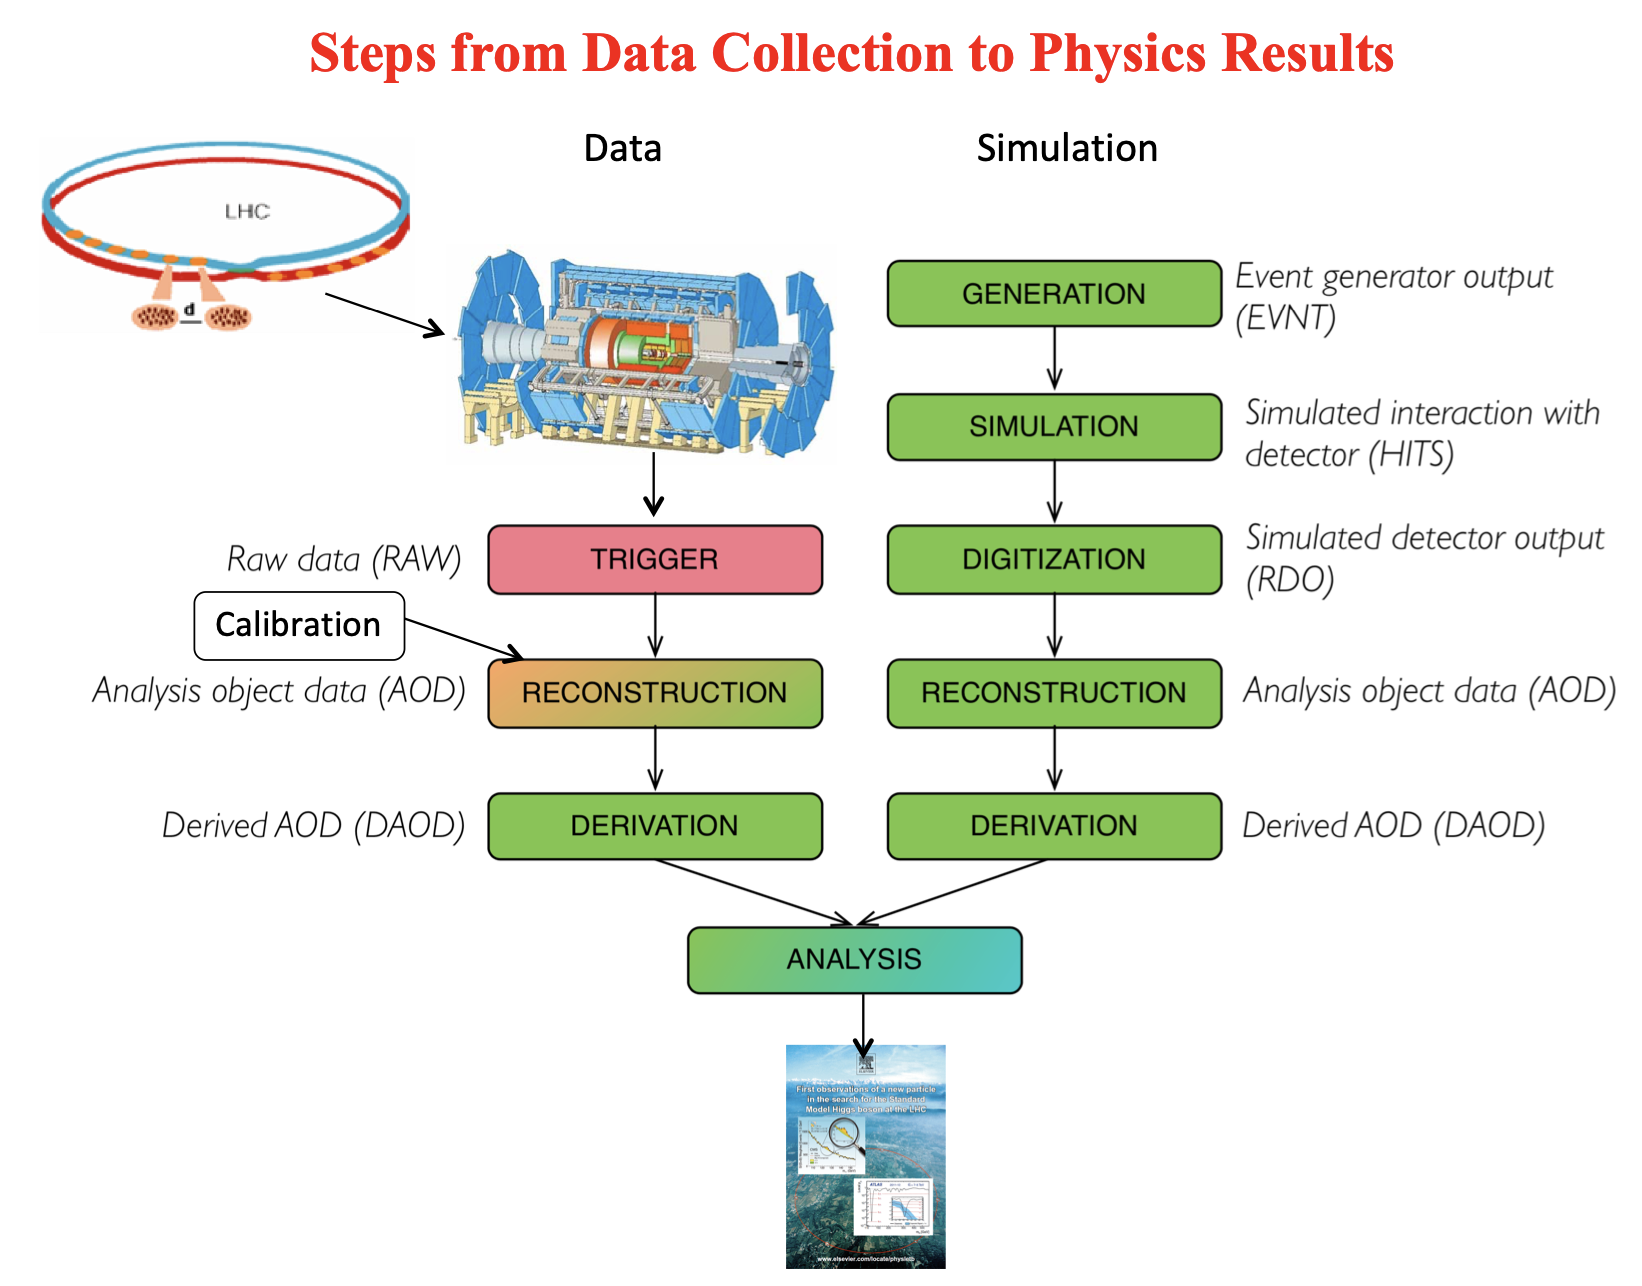
\includegraphics[width=\linewidth]{Figures/atlas/data_col_phys.png}
    \caption{Figure describing the steps to take for data collection at ATLAS, fetched from \href{https://indico.cern.ch/event/1159574/timetable/?view=standard}{Hybrid ATLAS Induction Day + Software Tutorial workshop}, part
    \href{https://indico.cern.ch/event/860971/contributions/3672974/attachments/1972049/3280896/Atlas_computing_data_preparation_jan20.pdf}{Computing and Data preparation}, 
    held by S.M Wang \cite{Wang:2707056} . }
    \label{fig:atlas_data_col_phys}
\end{figure}

